\documentclass[11pt]{article}
\pdfoutput=1 % compile with pdfLaTeX (three runs)

% ---------------------------------------------------------------- encoding and fonts
\usepackage[T1]{fontenc}
\usepackage[utf8]{inputenc}
\usepackage{lmodern}
\usepackage[american]{babel} % the paper is in American English: hyphenation patterns to match
\usepackage{textcomp}
\usepackage{amsmath,amssymb}
\usepackage[safe]{tipa}
% tipa has no Latin Modern version: take its Computer Modern glyphs (the design LM is based on)
\DeclareFontFamily{T3}{lmr}{}
\DeclareFontShape{T3}{lmr}{m}{n}{<->ssub * cmr/m/n}{}
\DeclareFontShape{T3}{lmr}{m}{it}{<->ssub * cmr/m/sl}{}
\DeclareFontShape{T3}{lmr}{m}{sl}{<->ssub * cmr/m/sl}{}
\DeclareFontShape{T3}{lmr}{bx}{n}{<->ssub * cmr/bx/n}{}
\DeclareFontShape{T3}{lmr}{b}{n}{<->ssub * cmr/bx/n}{}
\DeclareFontShape{T3}{lmr}{bx}{it}{<->ssub * cmr/bx/sl}{}
% make the IPA glyphs copy and search as Unicode in the PDF (tipa's glyph names are ASCII letters)
\input{glyphtounicode}
\pdfgentounicode=1
\makeatletter
\@for\tipa@font:={tipa8,tipa9,tipa10,tipa12,tipasl8,tipasl9,tipasl10,tipasl12}\do{%
  \pdfglyphtounicode{tfm:\tipa@font/at}{0259}%     schwa
  \pdfglyphtounicode{tfm:\tipa@font/P}{0294}%      glottal stop
  \pdfglyphtounicode{tfm:\tipa@font/E}{025B}%      open e
  \pdfglyphtounicode{tfm:\tipa@font/O}{0254}%      open o
  \pdfglyphtounicode{tfm:\tipa@font/colon}{02D0}}% length mark
\makeatother
% IPA and symbols that pdfLaTeX's utf8 input does not cover by default
\DeclareUnicodeCharacter{0259}{\textschwa}
\DeclareUnicodeCharacter{0294}{\textglotstop}
\DeclareUnicodeCharacter{025B}{\textepsilon}
\DeclareUnicodeCharacter{0254}{\textopeno}
\DeclareUnicodeCharacter{02D0}{\textlengthmark}
\DeclareUnicodeCharacter{2205}{\ensuremath{\varnothing}}
\DeclareUnicodeCharacter{2265}{\ensuremath{\geq}}
\DeclareUnicodeCharacter{2212}{\ensuremath{-}}
\DeclareUnicodeCharacter{0394}{\ensuremath{\Delta}}
\DeclareUnicodeCharacter{03B4}{\ensuremath{\delta}}

% ---------------------------------------------------------------- page layout
\usepackage[a4paper,top=25mm,bottom=28mm,left=28mm,right=28mm]{geometry}
\usepackage[final]{microtype}
\frenchspacing
\setlength{\emergencystretch}{1.5em}
\clubpenalty=10000 \widowpenalty=10000 \displaywidowpenalty=10000 % no single lines stranded at page breaks
\usepackage{xcolor}
\definecolor{linkblue}{HTML}{1F4E8C}

% ---------------------------------------------------------------- floats, tables, captions
\usepackage{graphicx}
\setkeys{Gin}{keepaspectratio}
\usepackage{booktabs,array,tabularx}
\usepackage{etoolbox}
% (\hbadness: rows can fall a few sp short of the width when the shares round; cells are ragged-right anyway)
\AtBeginEnvironment{tabularx}{\small\renewcommand{\arraystretch}{1.18}\hbadness=10000 }
% L{s}: ragged-right column taking share s of the table's width (the shares in a table add up to its column count)
\newcolumntype{L}[1]{>{\raggedright\arraybackslash\hsize=#1\hsize\linewidth=\hsize}X}
% \hd{...}: header cell, bottom-aligned so headers of different lengths sit on the same rule
\newcommand{\hd}[1]{\begin{minipage}[b]{\linewidth}\raggedright #1\end{minipage}}
\AtBeginEnvironment{table}{\centering}
\usepackage{caption}
\captionsetup{font=small, labelfont=bf, labelsep=period, justification=raggedright, singlelinecheck=false, skip=6pt}
\captionsetup[table]{position=top}
\usepackage{float}
\floatplacement{figure}{htbp}
\renewcommand{\topfraction}{0.9}
\renewcommand{\textfraction}{0.08}
\renewcommand{\floatpagefraction}{0.75}
\setcounter{topnumber}{3}
\setcounter{totalnumber}{4}
% float-only pages: stack the floats from the top instead of spreading them over the page
\makeatletter
\setlength{\@fptop}{0pt}
\setlength{\@fpsep}{\floatsep}
\setlength{\@fpbot}{0pt plus 1fil}
\makeatother

% ---------------------------------------------------------------- lists
\usepackage{enumitem}
\setlist{itemsep=2pt, parsep=0pt, topsep=4pt}

% ---------------------------------------------------------------- citations: author-year, no comma before the year
\usepackage[round]{natbib}
\setcitestyle{aysep={},yysep={,}}
\setlength{\bibhang}{1.4em}
\setlength{\bibsep}{3pt}
\renewcommand{\bibfont}{\small}

% ---------------------------------------------------------------- links
\usepackage[hyphens]{xurl}
\usepackage{hyperref}
\hypersetup{pdftitle={Where do Idaté and Lakalei belong? A pre-registered lexical-phylogenetic test of two classifications of Timor's Austronesian languages},
  pdfauthor={Dennis Crowley}, pdflang={en-US}, colorlinks=true, linkcolor=linkblue, citecolor=linkblue, urlcolor=linkblue,
  pdfkeywords={Timor, Austronesian, subgrouping, computational phylogenetics, language contact, pre-registration}}

% DOIs in the references, as links
\newcommand{\doi}[1]{doi:\href{https://doi.org/#1}{\nolinkurl{#1}}}

\title{Where do Idaté and Lakalei belong? A pre-registered lexical-phylogenetic test of two classifications of Timor's Austronesian languages}
\author{Dennis Crowley\thanks{Data, code, protocol and results: \url{https://github.com/DenC-dev/liabut}.}\\[2pt]
  \normalsize Phaistos Labs}
\date{November 2026}

\begin{document}

\maketitle

\begin{abstract}
\noindent Hull places Idaté and Lakalei with Mambae, Kemak and Tokodede; Grimes and Edwards (2026) place them in Timor-Babar, apart from Central Timor, on the evidence of *p lenition. This paper tests what LexiRumah's basic vocabulary says, with a protocol written before analysis, two replications with predictions declared in advance, and a second round governed by a decision rule declared before it was run. It gives Idaté, Lakalei, Welaun, Habu, Midiki and Helong what are, to our knowledge, their first cognate-based computational placements; all had been classified before by the comparative method. What the data show: model-based lexical trees place Lakalei-Idate beside Central Timor and never with the Eastern Timor languages, and seven outgroups put the root outside that pair under every outgroup set and missing-data treatment tried. But support depends on cognate coding and taxon choice (0 to 98\%), Idaté alone splits its support between Central Timor and neighboring Habu, shared innovations no longer favor Central Timor over Habu once retentions are removed, and no topology test rejects either placement after correction, although a Bayes factor under a no-borrowing model favors Central Timor (ln BF +11.8). *p lenition fits Grimes and Edwards's tree better whenever restoring *p costs at least twice as much as losing it, and the sound changes never fit the lexical tree uniquely best. By the declared rule, the question is unresolved by the vocabulary. What the data suggest: a history shaped by contact or a dialect linkage as well as descent, with Lakalei resembling Mambae and Idaté resembling Habu, each its neighbor. What remains unknown: whether either classification's subgroup is historically correct. That needs specialist review of the 47 decisive cognate comparisons, regular correspondences from fuller word lists, and independent replication; the materials for each are public.

\medskip
\noindent\textit{Keywords:} Timor; Austronesian; subgrouping; computational phylogenetics; language contact; pre-registration
\end{abstract}

\section{Introduction}

Two classifications of the Austronesian languages of Timor disagree about where Idaté and Lakalei belong. \citet{hull1998,hull2001a} groups all of Timor's Austronesian languages as \emph{Timoric}, split into \emph{Ramelaic} (Mambae, Kemak, Tokodede and Idalaka, that is Idaté and Lakalei) and \emph{Fabronic} (Tetun, Habun, the Kawaimina languages, Galoli, Wetarese, Dawan and Bekais or Welaun), and proposes that Ramelaic descends from Old Idalaka (as summarized by \citealt{albuquerque2009}). Carvalho (2001, cited in \citealt{fogaca2015}) proposed the same two-way split. \citet{edwards2019,edwards2021} and \citet{grimes2026}, building on \citet{donohue2008}, instead make \emph{Central Timor} (Mambae, Kemak, Tokodede and Welaun) a separate branch of Malayo-Polynesian, defined by *ŋ \textgreater{} *g, and place every other Austronesian language of Timor, Idaté and Lakalei included, in \emph{Timor-Babar}, defined by *p \textgreater{} *h.\footnote{\citet{grimes2026} do not discuss Hull's classification.}

The disagreement comes down to two questions. \textbf{C1}: does Lakalei-Idate (Hull's Idalaka) share a common ancestor with Central Timor, as in Hull, or with the other Timor-Babar languages, as in Grimes and Edwards? \textbf{C2}: is Welaun a dialect of Tetun, as \citet{hull1998} first had it, or a Central Timor language \citep{edwards2019}? \citet{hull2003} himself withdrew the Tetun-dialect claim, so C2 is the weaker contrast, and this paper concentrates on C1.

Grimes and Edwards argue from historical phonology, supported by morphosyntax and the lexicon. That sets two limits on what vocabulary can say. A subgroup defined by a shared sound change is not refuted by a lexical tree that fails to recover it, because shared vocabulary mixes inheritance, shared retention and borrowing \citep{blust2000,heggarty2010}. And if Central Timor is a primary branch, a tree with Lakalei-Idate beside Central Timor and a tree with Lakalei-Idate as the first branch of Timor-Babar can be the same unrooted tree, so C1 is partly a question about the root.

\textbf{What is new here, stated precisely.} \citet{gray2009}, to our knowledge the only earlier computational phylogeny that includes Timor's Austronesian languages, includes Tetum, Mambai and Kemak but none of Idaté, Lakalei, Welaun, Habu, Midiki or Helong, which are absent from ABVD. Three kinds of novelty need separating:

\begin{itemize}
\item \emph{Computational phylogenetic placement.} To our knowledge this paper gives these six languages their first cognate-based computational phylogenetic placement.
\item \emph{Systematic cognate analysis.} This is not new. LexiRumah codes cognates automatically for all of them \citep{kaiping2019}, and \citet{grimes2026} compare them systematically by the comparative method, with reconstructions and regular correspondences.
\item \emph{Historical classification.} This is not new either. All six are classified by \citet{hull1998,hull2001a} and by \citet{grimes2026}, and Welaun by \citet{edwards2019}, who also gives lexical percentages for it.
\end{itemize}

\textbf{Design.} The study has a protocol written before any analysis, two replications with predictions declared in advance, a second round of analyses governed by a decision rule declared before it was run, and a larger body of exploratory work. \citet{robinson2012} used lexical phylogenetics where sound changes had left the subgrouping of Alor-Pantar unresolved; here the question is the reverse, whether the vocabulary can arbitrate between a classification built on sound changes and an older one. The paper distinguishes throughout between what the data show, what they suggest, and what remains unknown, and closes on each in turn. The exploratory analyses that do not bear directly on C1 are in the \hyperref[supplement]{Supplement}.

\section{Data}

\begin{table}[tbp]
\caption{Data sources. All are CC BY 4.0. The repository's
\texttt{PROVENANCE.md} gives versions, commits and permissions, and
\texttt{DATA\_DICTIONARY.md} documents every lect, character, cognate
assignment and exclusion code.}
\label{tab:sources}
\begin{tabularx}{\linewidth}{@{}L{0.951}L{1.317}L{0.732}@{}}
\toprule
\hd{Source} & \hd{Contents} & \hd{Use} \\
\midrule
LexiRumah 3.0.1 \citep{kaiping2019} & 70 Timor-region lects, 152 concepts & Main lexical data (D1) \\
Austronesian Basic Vocabulary Database, ABVD \citep{greenhill2008} & 30 lects with expert cognate judgments; Proto-Malayo-Polynesian (PMP) forms; Tagalog, Buginese, Uma, Kambera, Bima, Manggarai & Validation (D2); PMP etyma; outgroups for rooting \\
\citet{grimes2026}, LaTeX source & 257 comparative tables (250 with language rows), 14,401 forms, reflexes marked by the authors & Sound-change atlas and characters \\
Austronesian Comparative Dictionary \citep{acd} & Etyma from Proto-Austronesian (PAN) to Proto-Central Malayo-Polynesian (PCMP) & Etymological check \\
\bottomrule
\end{tabularx}
\end{table}

Each lect (a word list for one language variety) needed at least 100 of the 152 concepts. Forms that look like Indonesian loans (against LexiRumah's Indonesian glosses) or Portuguese loans (against the Intercontinental Dictionary Series; \citealt{keycomrie2023}) are removed from the primary data; forms that look like Tetun loans, and Papuan-side forms resembling Austronesian ones, are removed only in sensitivity variants. The Idaté and Lakalei lists come from surveys by \citet{klamer2002} and \citet{dawson2014}, not from Edwards or Grimes. Figure~\ref{fig:map} shows the 24 lects used in the model-based analyses, one per language. Names follow LexiRumah, with Idaté for Idate, Habu for Habun, Tetun for Tetum and Welaun for Bekais.

\begin{figure}
\centering
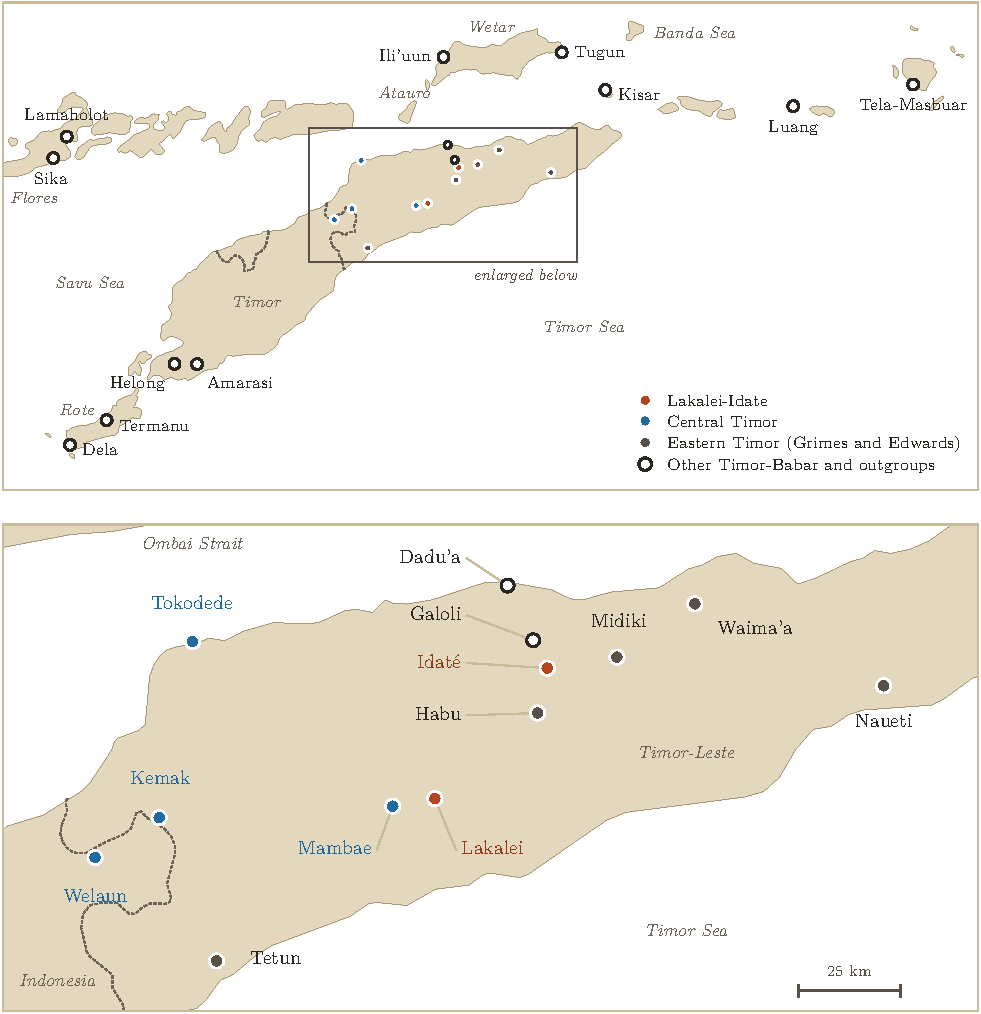
\includegraphics[width=\textwidth]{figures/map.pdf}
\caption{The 24 lects used in the Bayesian and maximum-likelihood analyses, one per language. Lakalei-Idate (red) lies between Central Timor (blue) and the Eastern Timor languages of Grimes and Edwards (dark gray); the dashed line is the border between Timor-Leste and Indonesia. Coordinates from LexiRumah; coastlines from Natural Earth.}
\label{fig:map}
\end{figure}

\section{Design: what each analysis can establish}

The protocol was written on October 10, 2026, before any analysis. Fourteen dated addenda, kept in the repository's \texttt{PROTOCOL.md}, extended it. All but Addendum 1 were committed before the analyses they govern; Addendum 1 re-scored the gate after it had failed (Table~\ref{tab:deviations}), and one exploratory analysis (E4) was never declared. Each addendum was written after the results of the previous ones had been seen. The analyses therefore fall into four classes that can establish different things (Table~\ref{tab:classes}).

\begin{table}[tbp]
\caption{What each class of analysis can establish.}
\label{tab:classes}
\begin{tabularx}{\linewidth}{@{}L{0.809}L{1}L{1.191}@{}}
\toprule
\hd{Class} & \hd{Analyses} & \hd{What it can establish} \\
\midrule
Original pre-registered tests & Steps 1 to 8: distance trees with concept bootstraps; decision rule of 70\% support in both UPGMA and neighbor-joining (NJ) trees, on the primary data and two screened variants & Results evaluated under the initial protocol, subject to the deviations in Table~\ref{tab:deviations} \\
Pre-declared replications & Addendum 9, predictions P1 to P5 (E26, E28) & Tests of predictions stated before those analyses were run \\
Second-round analyses & Addendum 12: E40 (root), E44 (Lakalei-Idate kept together), E45 (topology tests), E46 (cleaned, polarized innovations), under a decision rule declared in advance & Tests governed by an explicitly declared rule, written after earlier results had been seen \\
Exploratory analyses & Everything else, including the Bayes factors, the sound-change scoring, the contact models and Addenda 13 and 14 & Hypothesis-generating evidence and robustness checks, not independent confirmation \\
\bottomrule
\end{tabularx}
\end{table}

\textbf{Primary analysis.} Of the confirmatory components, the second round's rule bears most directly on C1, and it is treated as the primary analysis, although it was declared after the first round's results were known. It reports Central Timor as lexically supported only if four conditions all hold (Table~\ref{tab:primary}), and Grimes and Edwards's placement only if Timor-Babar is a rooted clade or the root sits on the Central Timor stem. Six robustness checks accompany it: the independent word lists, each member of Lakalei-Idate alone, other cognate codings, removing Tetun or sets shared with Papuan languages, other outgroups and missing-data treatments for the root (E57), and other assumptions about the reversibility of sound change (E56). The remaining analyses, numbered E1 to E57 as in the repository and listed in Table~\ref{tab:register}, are in the \hyperref[supplement]{Supplement}.

\begin{table}[tbp]
\caption{Deviations from the original protocol.}
\label{tab:deviations}
\begin{tabularx}{\linewidth}{@{}L{0.766}L{1.234}@{}}
\toprule
\hd{Protocol} & \hd{What happened} \\
\midrule
Gate: all four conditions under the v1 rules & G2 failed. Addendum 1 made G2 relative to the expert benchmark the same day, before any contested clade was scored \\
Steps 5 to 8 blind to the Timor topology & While diagnosing the gate, the analyst saw the full UPGMA tree, Timor lects included \\
Step 7: BEAST2, relaxed clock, Yule prior & Replaced by unrooted MrBayes (Addendum 2.4); a relaxed clock was run only in the second round \\
Step 7: Hull-constrained against Edwards-constrained runs, 100 stepping stones & Each clade forced against forbidden, 50 stones; direct comparisons added in the second round \\
Step 8: the decision uses bootstrap rules and a Bayes factor & The bootstrap conditions failed first, so the Bayes factor never decided anything \\
\bottomrule
\end{tabularx}
\end{table}

\textbf{Multiple testing.} Three families of tests were run. Eleven approximately unbiased (AU) topology tests (E6, E36, E45) are corrected together by Holm's \citeyearpar{holm1979} method; none rejects any placement (smallest adjusted p = 0.12). Forty triplet tests of contact (E18, E24) are corrected together; only Welaun's excess sharing with Tetun in borrowable words survives (E25). The remaining exploratory results are reported as estimates, not as tests, and the few uncorrected p-values in the \hyperref[supplement]{Supplement} are marked as such. None of the conclusions below rests on an uncorrected p-value.

\section{Methods}

\textbf{Cognates.} LexStat (threshold 0.55) with Infomap clustering in LingPy 2.6.14 \citep{list2017}. Scored against ABVD's expert judgments, it reaches a B-cubed F of 0.81 (precision 0.88, recall 0.75). Automatic cognates suffice for phylogenetic reconstruction in some families but not all \citep{rama2018}, so four other codings are used as checks: sound-class alignment (SCA), LexStat at two other thresholds, a consensus of five codings (E27) and morpheme-level partial cognates \citep[E51;][]{list2016}.

\textbf{Trees.} Each cognate set is one binary character; a lect without the concept is coded missing. The 24 lects give 1,353 characters. MrBayes 3.2.7a \citep{ronquist2012} used the restriction model with no all-absent sites, gamma rate variation and exponential(10) branch lengths; IQ-TREE 2.3.6 \citep{minh2020} used GTR2+FO+G4 with 1,000 ultrafast bootstrap replicates \citep[UFBoot;][]{hoang2018}, conventionally read as support only at 95 or above.

\textbf{Rooting.} A root needs outgroups that are certainly outside the ingroup, close enough to share cognates with it, and free of its contact history \citep{nixon1993}. No single choice meets all three, so three kinds were used, from ABVD, coded together with the Timor data (E40): three Western Malayo-Polynesian languages (Tagalog, Buginese, Uma), outside Central Malayo-Polynesian on every classification but distant; three Central Malayo-Polynesian languages of Sumba, Sumbawa and western Flores (Kambera, Bima, Manggarai), closer but in the same Lesser Sunda contact sphere; and Blust's PMP reconstruction \citep{blust2013} as a pseudo-taxon. A reconstruction is a risky taxon. It is built partly from the languages being rooted and their relatives; it has no borrowings, no gaps of the usual kind and one etymon per meaning; and its forms lean toward conservative, well-documented languages, which can pull the root toward conservative lineages. The PMP-only rooting is therefore read as a check, never alone, and E57 reruns the root without it, without each other outgroup in turn, with missing data coded as absence, and on the 99 concepts attested in all seven outgroups. A relaxed clock (E41) gives a root without outgroups.

\textbf{Retentions and innovations.} A shared word is evidence for a subgroup only if it is a shared innovation; a shared retention says nothing. Each cognate set is classed as a PMP retention or an innovation by its distance from ABVD's PMP word after substituting each lect's regular reflexes (rule R2, balanced accuracy 0.79 against ABVD's experts; a learned classifier did not beat it, E54). The sets behind the decisive counts were then checked: by an internal mock review (not a specialist one), against strict Austronesian Comparative Dictionary etyma (E35) and against Grimes and Edwards's own tables (E37). Sets also present in Flores, Rote-Meto or Wetar are set aside as probably old (polarization). Every reclassification has a reason code in the repository's audit trail (\texttt{derived/audit/exclusions.csv}), and the 47 decisive sets are tabulated with their forms, etyma and audit entries for specialist review (\texttt{derived/audit/decisive\_comparisons.csv}).

\textbf{Contact.} The triplet test counts, for three groups, the concepts on which exactly two share an innovation \citep[the lexical counterpart of ABBA-BABA;][]{green2010,durand2011}, separately on the 60 Leipzig-Jakarta concepts \citep{tadmor2009} and on the rest, with nulls simulated under unequal rates (E31) and a calibration of the decision rule (E46).

\textbf{Sound changes.} The marked reflexes in Grimes and Edwards's tables were turned into an expert reflex atlas (Figure~\ref{fig:sounds}); LexiRumah forms aligned to PMP gave an automatic atlas, agreeing on 94\% of tokens. Eleven changes were coded as binary characters and scored on three rooted trees (the lexical tree H, Lakalei-Idate + Eastern Timor G, and Grimes and Edwards's top split GE) by Fitch \citep{fitch1971}, Camin-Sokal \citep{camin1965} and Dollo \citep{farris1977} parsimony, and by \citet{sankoff1975} parsimony with the cost of restoring a lost sound varied from a tenth to a thousand times the cost of losing it (E56).

\section{Results}

\subsection{Pre-registered tests and replications}

Only low-level groups reach the 70\% bar in both distance trees: Lakalei-Idate, Kawaimina, Wetar-Atauro, Nuclear Rote, Kisar-Luang, Kisar-Roma and Babar, and groups nested within them. Hull's Ramelaic scores 22\% (UPGMA) and 55\% (NJ); Fabronic, Timor-Babar and Eastern Timor 0 to 3\%. The pre-registered decision is \textbf{unresolved} for both C1 and C2. The rule relies on UPGMA, which assumes a clock and is misled by unequal rates \citep{blust2000}, so it had little chance of resolving higher-level groups. The replications partly failed. Across 351 combinations of dialect lists (E26), Lakalei-Idate + Nuclear Central Timor (Mambae, Kemak, Tokodede) was the largest stable-vocabulary pair against Habu and Kawaimina in every combination but against Tetun in only 47\% (86\% with Tetun Suai, 9\% with Tetun Dili, the lingua franca). On lists collected independently of Grimes and Edwards (E28), the prediction failed against Tetun by one concept (45 to 44), while the prediction that Timor-Babar and Lakalei-Idate + Eastern Timor get at most 5\% held (0\%).

\subsection{The primary analysis}

\begin{table}[tbp]
\caption{The primary analysis: the second round's decision rule for C1.
Grimes and Edwards's placement would have been reported as lexically
supported if Timor-Babar were a rooted clade (posterior ≥ 0.95), or if
the root sat on the Central Timor stem (≥ 0.95) and Lakalei-Idate +
Eastern Timor were not rejected; neither happened (posterior 0.00 for
both).}
\label{tab:primary}
\begin{tabularx}{\linewidth}{@{}L{2.056}L{0.722}L{0.222}@{}}
\toprule
\hd{Condition for reporting Central Timor (Addendum 12)} & \hd{Result} & \hd{Met?} \\
\midrule
1. Root: Lakalei-Idate + Central Timor a rooted clade, MrBayes posterior ≥ 0.95, and UFBoot ≥ 95 in two of three outgroup sets & Posterior 1.00; UFBoot 98, 98 and 97 & Yes \\
2. Lakalei-Idate kept together: UFBoot ≥ 95 with Central Timor on both list sets & 70 (primary), 98 (independent) & No \\
3. Lakalei-Idate + Eastern Timor and Timor-Babar both rejected after Holm, root held by outgroups & Not rejected (adjusted p 0.06 and 0.11 for Timor-Babar; 0.52 and 0.28 for the eastern placement, within E45) & No \\
4. Cleaned, polarized stable pairing largest against Tetun, Habu and Kawaimina, with the tree-pair rule producing it under G in under 20\% & Fails against Habu (10 to 12) & No \\
\bottomrule
\end{tabularx}
\end{table}

By the rule declared before the second round, \textbf{C1 is unresolved by the vocabulary}. Only the root condition holds. The next sections take each condition in turn and show why the evidence divides.

\subsection{The root}

\begin{table}[tbp]
\caption{Where the root falls. Each tree is reduced to the 24 lects and
rooted on Tagalog (Buginese without Tagalog; Kambera for the near set;
PMP for PMP alone). Rows in italics are the E57 sensitivity runs, all
UFBoot. In the relaxed clock the remaining 0.47 is spread over other
branches, 0.17 of it on Kisar-Luang-Tela-Masbuar. Timor-Babar is a
rooted clade in none (0.00 throughout).}
\label{tab:root}
\begin{tabularx}{\linewidth}{@{}L{2.222}L{0.695}L{0.695}L{0.695}L{0.693}@{}}
\toprule
\hd{Analysis} & \hd{Root on Flores} & \hd{Root on Rote-Meto + Helong} & \hd{Root on Central Timor stem} & \hd{Lakalei-Idate + Central Timor a rooted clade} \\
\midrule
All seven outgroups, MrBayes & 0.93 & 0.07 & 0.00 & 1.00 \\
All seven outgroups, UFBoot & 0.87 & 0.12 & 0.00 & 0.98 \\
Far outgroups only & 0.16 & 0.77 & 0.00 & 0.98 \\
Near outgroups only & 0.94 & 0.03 & 0.00 & 0.98 \\
PMP only & 0.04 & 0.70 & 0.00 & 0.97 \\
Relaxed clock, no outgroups & 0.11 & 0.42 & 0.00 & 0.96 \\
\emph{E57: without Tagalog / Buginese / Uma} & \emph{0.89 / 0.87 / 0.83} & \emph{0.10 / 0.12 / 0.15} & \emph{0.00} & \emph{0.97 / 0.96 / 0.97} \\
\emph{E57: without Kambera / Bima / Manggarai} & \emph{0.81 / 0.92 / 0.46} & \emph{0.17 / 0.07 / 0.51} & \emph{0.00} & \emph{0.95 / 0.97 / 0.98} \\
\emph{E57: without PMP} & \emph{0.96} & \emph{0.03} & \emph{0.00} & \emph{0.97} \\
\emph{E57: missing data coded as absence} & \emph{0.36} & \emph{0.60} & \emph{0.00} & \emph{0.86} \\
\emph{E57: only the 99 concepts attested in all seven outgroups} & \emph{0.83} & \emph{0.13} & \emph{0.00} & \emph{0.96} \\
\bottomrule
\end{tabularx}
\end{table}

In no analysis, and under no outgroup choice or missing-data treatment, does the root fall on the Central Timor stem (Table~\ref{tab:root}; Figure~\ref{fig:tree}). It falls on the Flores or the Rote-Meto + Helong branch; which of the two depends on the outgroups and on how missing data are coded, but Central Timor and Lakalei-Idate stay on the same side. This rules out one reconciliation, that the lexical tree is Grimes and Edwards's tree rooted in a different place.

It does not establish an inherited subgroup. A rooted clade in a lexical tree means that the languages in it share more cognate presences and absences with each other than with the outgroups, in a pattern the model attributes to descent. It becomes evidence for a subgroup only if those shared features are innovations, inherited rather than borrowed, and not retentions concentrated in conservative lineages. The outgroups also attach by lexical similarity, so contact across the Savu Sea, or Rote-Meto's conservatism, could pull them west.

\begin{figure}
\centering
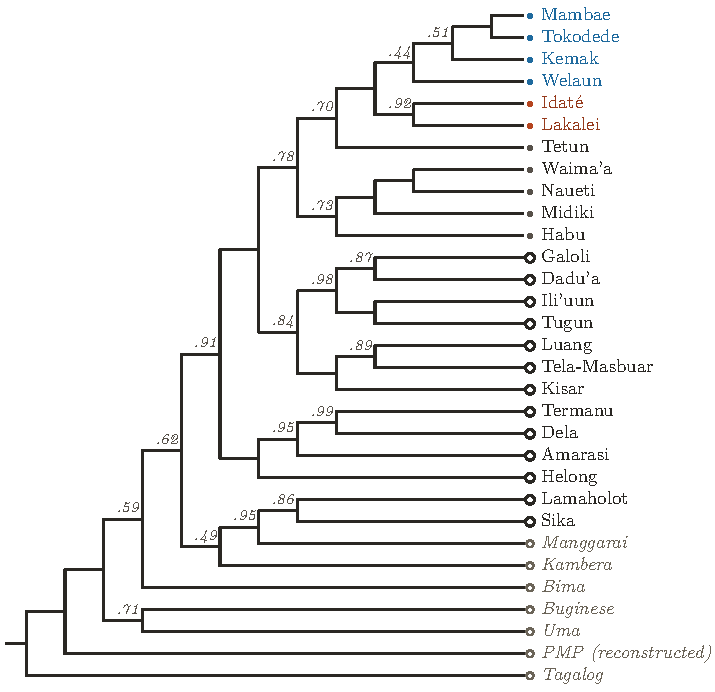
\includegraphics[width=0.8\textwidth]{figures/tree.pdf}
\caption{Consensus tree (all compatible splits) of the Bayesian analysis with seven outgroups (gray), 31 lects and 1,599 cognate characters coded together (E40), rooted on Tagalog and drawn as a cladogram. Numbers are posterior probabilities; unlabeled nodes exceed 0.99.}
\label{fig:tree}
\end{figure}

\subsection{How robust is the placement?}

\begin{table}[tbp]
\caption{Robustness checks on the placement of Lakalei-Idate. On the
independent lists Central Timor has no Welaun. Other codings are in the
Supplement.}
\label{tab:robust}
\begin{tabularx}{\linewidth}{@{}L{2.3}L{0.7}L{0.7}L{0.65}L{0.65}@{}}
\toprule
\hd{UFBoot \%} & \hd{With Central Timor} & \hd{With Nuclear Central Timor} & \hd{With Eastern Timor} & \hd{With Habu} \\
\midrule
Primary lists, Lakalei-Idate kept together & 70 & 41 & 0 & 0 \\
Independent lists, kept together & 98 & 98 & 0 & 0 \\
Primary lists, Idaté alone & 52 & 3 & 2 & 38 \\
Primary lists, Lakalei alone & 84 & 75 & 0 & 0 \\
Without Tetun (E48) & 94 & 8 & 1 & 2 \\
Without 132 sets shared with Papuan lects (E48) & 46 & 51 & 0 & 0 \\
Consensus of five codings (E27) & 0 & 55 & 0 & \\
Partial cognates, kept together (E51) & 28 & 73 & 0 & 12 \\
LexiRumah's own cognates (E15) & 0 & & & 51 (Lakalei-Idate + Habu) \\
\bottomrule
\end{tabularx}
\end{table}

No coding, taxon set or list set puts Lakalei-Idate with Eastern Timor (0 to 7\%). Support for the Central Timor side varies from 0\% to 98\% with choices that should not matter historically (Table~\ref{tab:robust}; a check modeled on \citealt{kaiping2022}): which cognate coding is used, whether the pair is forced together, which lists represent the languages. Lakalei on its own is Central Timor-like in every run; Idaté on its own splits its support between Central Timor (52) and Habu (38), its neighbor 5 to 11 km away, though not on the independent lists (79 and 13). Removing Tetun raises the Central Timor link, so Tetun loans are not what holds it together; removing the sets shared with Papuan languages lowers it, and Mambae, Kemak, Welaun, Idaté and Lakalei each share 40 to 49 sets with Papuan lects against 30 to 37 for Tokodede and the Eastern Timor languages, so some of the link may run through shared contact with Bunak.

\subsection{Topology tests and Bayes factors}

\begin{table}[tbp]
\caption{Topology tests. AU tests \citep{shimodaira2002} use 10,000 RELL
replicates, with the root held by the seven outgroups and Lakalei-Idate
kept together; the parametric bootstrap (SOWH) uses 100 replicates. All
eleven AU tests of the project are in the \hyperref[supplement]{Supplement}. The direct
Bayesian comparison of the same two placements gives ln BF +11.8 for
Lakalei-Idate + Central Timor (E47).}
\label{tab:topology}
\begin{tabularx}{\linewidth}{@{}L{2.1}L{0.7}L{0.45}L{0.5}L{1.25}@{}}
\toprule
\hd{Constrained tree} & \hd{Lists} & \hd{Test} & \hd{p} & \hd{p, Holm over all eleven} \\
\midrule
Timor-Babar, rooted (E45) & Primary & AU & 0.011 & 0.12 \\
Lakalei-Idate + Eastern Timor (E45) & Primary & AU & 0.17 & 0.69 \\
Timor-Babar, rooted (E45) & Independent & AU & 0.022 & 0.22 \\
Lakalei-Idate + Eastern Timor (E45) & Independent & AU & 0.070 & 0.47 \\
Lakalei-Idate + Eastern Timor, Lakalei-Idate free to split (E38) & Primary & SOWH & 0.01 & \\
\bottomrule
\end{tabularx}
\end{table}

The Bayes factor and the corrected AU tests answer different questions, and the difference explains why one looks decisive and the other does not. The stepping-stone Bayes factor compares the average fit of two hypotheses over every tree and branch length consistent with each, assuming the model is correct. With 1,353 characters a small advantage per character accumulates into a large factor (+11.8), and because both hypotheses share the same model, which treats every shared word as inherited, the factor measures which placement that model prefers. The AU test asks whether the constrained tree fits significantly worse than the best tree, allowing for the variation one would see by resampling concepts and for having chosen the best of several candidates. Uncorrected it leans the same way (p = 0.011 to 0.17); after correction for eleven tests nothing is rejected. The two agree on the direction, toward Central Timor, and disagree on how far the preference survives sampling variation. The parametric bootstrap \citep[the Swofford--Olsen--Waddell--Hillis or SOWH test;][]{goldman2000} points the same way as the Bayes factor but is known to reject too readily when the model is misspecified \citep{buckley2002,susko2014}. The primary analysis required the corrected tests, so the direction is reported as a lean of the vocabulary under a no-borrowing model, not as a rejection of the eastern placement.

\subsection{Shared retentions and shared innovations}

\begin{table}[tbp]
\caption{Triplet counts on stable concepts (E46): concepts on which
exactly two of three groups share an innovation. LI is Lakalei-Idate;
NCT is Nuclear Central Timor (Mambae, Kemak, Tokodede). Counts are
summed over the combinations of lects in each group, so they exceed the
number of concepts.}
\label{tab:triplets}
\begin{tabularx}{\linewidth}{@{}L{2.636}L{0.454}L{0.454}L{0.456}@{}}
\toprule
\hd{Stable concepts, representative lists} & \hd{LI + NCT} & \hd{LI + X} & \hd{NCT + X} \\
\midrule
X = Tetun: as first counted & 21 & 12 & 10 \\
X = Tetun: retentions and errors removed & 10 & 5 & 6 \\
X = Tetun: also without sets found in Flores, Rote-Meto or Wetar & 8 & 5 & 0 \\
X = Habu: as first counted & 23 & 19 & 15 \\
X = Habu: retentions and errors removed & 12 & 12 & 4 \\
X = Habu: also without sets found in Flores, Rote-Meto or Wetar & 10 & 12 & 0 \\
X = Kawaimina: as first counted & 80 & 38 & 23 \\
X = Kawaimina: retentions and errors removed & 42 & 27 & 13 \\
X = Kawaimina: also without sets found in Flores, Rote-Meto or Wetar & 36 & 21 & 1 \\
\bottomrule
\end{tabularx}
\end{table}

Shared vocabulary only supports a subgroup where it is a shared innovation. As first counted, Lakalei-Idate's stable vocabulary pairs it with Nuclear Central Timor against all three eastern groups (Table~\ref{tab:triplets}). Of the 66 ``innovations'' reclassified after these checks, most were retentions: sets that continue an etymon older than any of the groups compared, such as PMP *(i)kahu `2sg' and *ikuR `tail', which the automatic rule had missed because the forms have changed a great deal. Three were coding errors (the two `wife' sets continue one etymon, PAN *b\textless in\textgreater ahi, which the coding split, and `who' grouped non-cognate forms) and one was doubtful (`dry'). Once these are removed, the pairing with Central Timor still beats Tetun and Kawaimina, ties with Habu, and loses to Habu once sets also found outside the triplet are set aside. Coded by morpheme instead (E51), and not cleaned by hand, the polarized counts lean further toward Tetun (18 against 10) and Habu (14 against 13), although loose morpheme coding also picks up Tetun loans inside compounds.

Calibration matters for reading these counts. With no borrowing, the rule ``Lakalei-Idate + Nuclear Central Timor strictly largest against all three groups'' is satisfied in only 21\% of datasets simulated on the lexical tree and 3\% on the eastern tree (15\% and 5\% with polarized counts), so it rarely produces the pattern by accident but usually misses it when it is true (E46). And unequal branch lengths alone produce large imbalances between the minority pairs: a naive Z ≥ 2 rule fires in 27\% of contact-free simulations (E31), so none of Lakalei-Idate's excess sharing in either direction is evidence of contact, and none is evidence against it.

Lakalei-Idate shares only a handful of innovations with exactly one other group (E17). After review two remain on the Central Timor side, `cry' (\emph{sɛro}, against \emph{tanis} \textless{} *taŋis almost everywhere else) and `spit', against nine on the eastern side that passed the automatic and etymological checks but have not been reviewed by hand. The comparison is uneven until they are. A test of regular sound correspondences in these sets (E52) found too few regular non-identity correspondences in these short lists (0 to 2 sound classes per lect pair) to tell loans from inheritance.

\subsection{The sound changes}

\textbf{The reflexes.} Table~\ref{tab:preflexes} gives the *p tokens for the focal languages in the two atlases word-initially, between vowels and before *u (\texttt{derived/audit/p\_reflexes.csv}). Mambae, Kemak and Tokodede keep a labial in every environment (p, or f in Mambae; one ʔ in Tokodede's *kəpit `narrow'). The eastern languages have h in every environment, with an occasional ʔ between vowels. Lakalei and Idaté have h word-initially (*pitu \textgreater{} \emph{hitu} `seven') but also loss (*pija \textgreater{} \emph{ila} `how much'), loss or h between vowels (*əpat \textgreater{} \emph{aːt} `four', *ma-nipis \textgreater{} \emph{mihis} `thin'), and w before *u (*hapuy \textgreater{} \emph{wai} `fire'). Welaun, a Central Timor language on every other count, has h, ʔ and loss. In *palu `hit' nearly every language has b (Tetun \emph{baku}, Lakalei \emph{baʔu}, Tokodede \emph{bɔnu}, Waima'a \emph{baː}), so that word is a separate development and counts for neither side.

\begin{table}[tbp]
\caption{Reflexes of PMP *p by environment, from the expert and
automatic atlases (Welaun's `fire' from its word list). Etyma in
brackets. Two automatic-atlas tokens are left out as probable alignment
artifacts: Lakalei \emph{ʔaːt} `four', whose ʔ is word-initial (the
expert atlas has loss), and Welaun \emph{sasaː} `what'
(*apa).}
\label{tab:preflexes}
\begin{tabularx}{\linewidth}{@{}L{1}L{1}L{1}L{1}@{}}
\toprule
\hd{Language} & \hd{Word-initial *p} & \hd{Between vowels} & \hd{Before *u} \\
\midrule
Mambae, Kemak, Tokodede & p, f (*pija, *puqun, *pusəj) & p, f (*əpat, *nipən, *nipay); ʔ once (*kəpit) & p, f (*hapuy) \\
Welaun & h (*piliq) & ∅ (*əpat), ʔ (*ma-nipis) & ʔ (*hapuy) \\
Lakalei & h (*pitu), ∅ (*pija) & ∅ (*əpat, *nipən), h (*ma-nipis) & w (*hapuy) \\
Idaté & h (*pitu), ∅ (*pija) & ∅ (*əpat), h (*ma-nipis) & w (*hapuy) \\
Tetun & h (*piliq) & h (*əpat, *nipən), ʔ (*ma-nipis) & \\
Habu & h (*pitu, *pija) & h (*əpat, *hipi), ʔ (*nipən) & h (*hapuy) \\
Kawaimina & h (*pitu, *pija, *punti, *panaq) & h (*əpat, *ma-nipis) & \\
Flores pair & p & p & p \\
\bottomrule
\end{tabularx}
\end{table}

\textbf{Four explanations.} The loss of *p in Lakalei-Idate could have four sources, which predict different things (Table~\ref{tab:explanations}).

\begin{table}[tbp]
\caption{Competing explanations for the loss of *p in
Lakalei-Idate.}
\label{tab:explanations}
\begin{tabularx}{\linewidth}{@{}L{0.8}L{1}L{1.12}L{1.08}@{}}
\toprule
\hd{Explanation} & \hd{What it predicts} & \hd{What the reflexes show} & \hd{Assessment} \\
\midrule
Shared innovation: one change in an ancestor of Lakalei-Idate and the eastern languages & The same outcome in the same environments in every daughter, apart from later changes and loans & The eastern languages have h throughout; Lakalei-Idate has h, loss and w & Compatible if Lakalei-Idate later lost h or rounded it before *u, both common changes; not uniquely predicted \\
Independent change in several lineages & Lenition in more than one branch, possibly with different outcomes & Welaun has h, ʔ and loss although it groups with Central Timor on every other count; p \textgreater{} h is among the most frequent lenitions \citep{kummel2007} & Plausible: it has happened at least twice on Timor \\
Restoration: Central Timor lenited *p and later restored it & Regular p in Central Timor continuing an earlier h & Regular p or f in 54 of 55 matched words, native ones included & Implausible: h \textgreater{} p is essentially unattested as a regular change, and borrowing could not restore p so regularly \\
Diffusion across varieties already separate & Spread by contact, outcomes varying by language, shared by neighbors regardless of subgroup & Welaun, in long contact with Tetun, has h; Lakalei-Idate's outcomes differ from the eastern ones; it borders Mambae (p) and Habu (h) & Plausible; fits a Timorese Sprachbund \citep{hull2001b,schapper2020}; cannot be told apart from a shared innovation with these data \\
\bottomrule
\end{tabularx}
\end{table}

Restoration is the least plausible of the four, which is why irreversible scoring is the appropriate default \citep{campbell2013}. The data cannot separate a shared innovation from diffusion or parallel change, and Welaun shows that parallel change has happened.

\textbf{How much the scoring assumption matters.} Table~\ref{tab:sankoff} scores the trees with the cost of a restoration set from a tenth of the cost of a change to a thousand times it (E56). For *p lenition the three trees tie when a restoration costs no more than a change. As soon as it costs twice as much, Grimes and Edwards's tree is cheapest, and at five times or more the lexical tree needs six origins against their two. Over all eleven characters, and over a fuller set of 36 characters from every reflex in the expert atlas (E53), the lexical tree is never the uniquely cheapest under any cost: Grimes and Edwards's tree wins when restorations are cheap, and the tree with Lakalei-Idate in Eastern Timor when they are costly, mainly because it groups Tetun with Habu and Kawaimina.

\begin{table}[tbp]
\caption{Sankoff parsimony costs on the three trees, rooted on the
Flores pair with the root state fixed at the PMP state (E56). H is the
lexical tree, G Lakalei-Idate + Eastern Timor, GE Grimes and Edwards's
top split. Bold marks the cheapest tree in each column; nothing is bold
where all three tie.}
\label{tab:sankoff}
\begin{tabularx}{\linewidth}{@{}L{1.13}L{0.956}L{0.956}L{0.958}@{}}
\toprule
\hd{Cost of a restoration, relative to a change} & \hd{*p lenition: H / G / GE} & \hd{Eleven characters: H / G / GE} & \hd{36 characters: H / G / GE} \\
\midrule
0.1 & 1.1 / 1.1 / 1.1 & 22.1 / 21.8 / \textbf{21.4} & 60.1 / 59.8 / \textbf{59.6} \\
0.5 & 1.5 / 1.5 / 1.5 & 31.5 / 31.5 / \textbf{30.0} & 85.5 / 85.5 / \textbf{85.0} \\
1 & 2 / 2 / 2 & 38 / 38 / \textbf{37} & 99 / \textbf{97} / 99 \\
2 & 3 / 3 / \textbf{2} & \textbf{44} / 45 / \textbf{44} & 107 / \textbf{100} / 103 \\
3 & 4 / 4 / \textbf{2} & 47 / 47 / 47 & 108 / \textbf{100} / 105 \\
5 or more & 6 / 4 / \textbf{2} & 49 / \textbf{47} / 50--51 & 108 / \textbf{100} / 107 \\
\bottomrule
\end{tabularx}
\end{table}

\begin{figure}
\centering
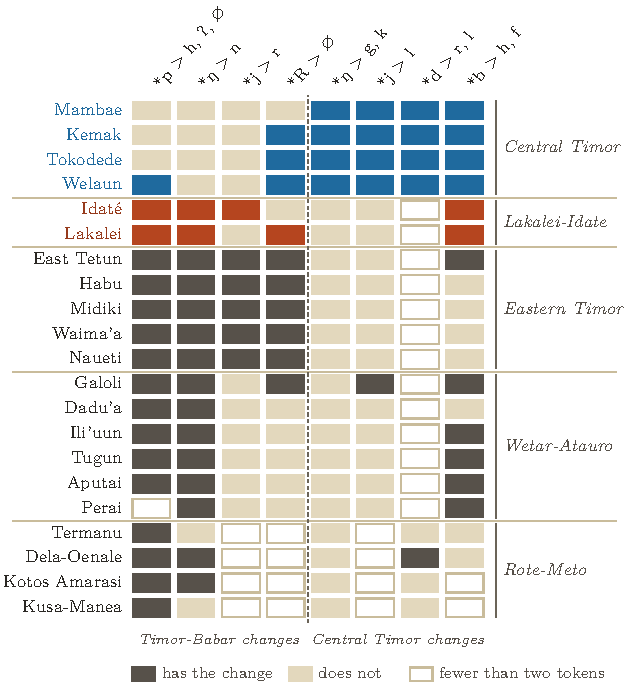
\includegraphics[width=0.8\textwidth]{figures/sounds.pdf}
\caption{Eight of the eleven sound-change characters (the other three are Hull's *b- \textgreater{} h and the loss of *k initially and medially), coded from the reflexes \citet{grimes2026} mark in their comparative tables, for the languages of Timor, Wetar-Atauro and Rote-Meto (Southwest Maluku is in the repository). Outlined cells rest on fewer than two expert tokens. The last column merges *b \textgreater{} h and *b \textgreater{} f, so it is not the same character as Hull's initial *b- \textgreater{} h.}
\label{fig:sounds}
\end{figure}

\subsection{Welaun (C2)}

Welaun goes with Central Timor in the model-based trees (posterior 0.86), its similarity to Tetun sits in borrowable words (the one contact signal that survives correction, E25), and compared directly Central Timor with Welaun beats Welaun + Tetun by ln BF +7.6 (E47). The pre-registered distance trees favor Welaun + Tetun (51\% and 59\%) and the consensus coding gives Central Timor with Welaun 0\%. Addendum 2.1 stated in advance that C2 cannot be settled lexically. Once borrowable vocabulary is set aside, the lexical evidence is consistent with \citet{edwards2019}.

\section{Discussion}

\subsection{Weighing the evidence}

\begin{table}[tbp]
\caption{The two classifications against the main lines of evidence for
C1.}
\label{tab:weighing}
\begin{tabularx}{\linewidth}{@{}L{1}L{1.08}L{1.2}L{0.72}@{}}
\toprule
\hd{Line of evidence} & \hd{Hull: Lakalei-Idate with Central Timor} & \hd{Grimes and Edwards: Lakalei-Idate in Timor-Babar} & \hd{Class} \\
\midrule
Pre-registered distance trees & Ramelaic 22\% and 55\%, below the bar & Timor-Babar 0 to 3\% & Pre-registered \\
Unrooted Bayesian tree & Lakalei-Idate + Central Timor 0.91 & Lakalei-Idate + Eastern Timor 0.00; compatible only with a root on the Central Timor stem & Exploratory \\
Root from outgroups and a relaxed clock & Rooted clade 0.86 to 1.00 & The root never falls on the Central Timor stem & Second round (met) \\
Lakalei-Idate kept together & 70\% (primary), 98\% (independent) & Not supported (0\%) & Second round (not met) \\
Topology tests after correction & Not rejected & Not rejected & Second round (not met) \\
Direct Bayes factor, no-borrowing model & Favored, ln BF +11.8 & Disfavored under that model & Exploratory \\
Shared innovations, cleaned and polarized & Ahead of Tetun and Kawaimina & Habu ahead (12 against 10) & Second round (not met) \\
Exclusive shared innovations & Two after review & Up to nine, not yet reviewed & Exploratory \\
*p lenition & Six origins if irreversible & Two origins if irreversible; tie if reversible & Exploratory \\
Fuller phonology, any reversibility & Never the cheapest tree & Cheapest when restorations are cheap & Exploratory \\
\bottomrule
\end{tabularx}
\end{table}

The vocabulary and the phonology point in different directions, and Table~\ref{tab:weighing} shows where the division lies. The lexical evidence leans toward Central Timor wherever it treats shared words as inherited, and weakens wherever retentions, coding choices and the internal split of Lakalei-Idate are taken into account. The sound-change evidence favors Grimes and Edwards wherever a lost *p is assumed not to come back, and never favors the lexical tree.

\textbf{Why the comparative method's evidence counts differently.} The two kinds of evidence are not interchangeable, and counting characters would mislead. A regular sound change is a structured character: it applies across the lexicon, is directional (p \textgreater{} h is common, h \textgreater{} p essentially unknown), and can be polarized without outgroups. A lexical character is cheap and noisy: each of the 1,353 sets records presence or absence in one meaning, cannot tell inheritance from shared retention or borrowing on its own, and is correlated with its neighbors through contact and differences in rate. So 1,353 lexical characters against one defining change is not a fair measure of the evidence on each side. Sound changes also spread by contact, however \citep{schapper2020}, and a single change is one character: Welaun shows that this one has arisen more than once. The comparative method's evidence here is strong in kind but thin in amount, and the lexical evidence is plentiful but needs the comparative method's checks to become a claim about subgroups.

\subsection{What the data show}

\begin{itemize}
\item Model-based lexical trees place Lakalei-Idate beside Central Timor and never with the Eastern Timor languages, and seven outgroups root the tree outside that pair under every outgroup set and missing-data treatment tried.
\item That support is sensitive to coding and taxon selection (0 to 98\%), Idaté on its own splits its support between Central Timor and Habu, and no topology test rejects either placement after correction.
\item Once identified retentions and errors are removed, Lakalei-Idate's shared stable innovations no longer favor Central Timor over Habu.
\item *p lenition fits Grimes and Edwards's tree better whenever a restoration costs at least twice a lenition; the sound changes never fit the lexical tree uniquely best.
\item Lexical trees here also miss about half of the subgroups that sound changes define and nobody disputes (E43), so a missing lexical Timor-Babar says little about Timor-Babar.
\end{itemize}

\subsection{What the data suggest}

The pattern fits a history shaped by contact or a linkage as well as by descent. Lakalei resembles Mambae, its neighbor 10 km away, and Idaté resembles Habu, 5 to 11 km away. A split network (E55) shows Lakalei-Idate with Central Timor in 47\% of resampled networks and Idaté with Habu in 45\%, and glottometry ties Lakalei-Idate about equally weakly to both sides. Such cross-cutting ties are what a dialect linkage leaves \citep{ross1988,francois2014}, and Grimes and Edwards already divide Wetar-Atauro into ``two overlapping subgroups''. Shared contact with Papuan neighbors may carry part of the Central Timor link; East Nusantara is a linguistic area in its own right \citep{klamer2008}. Lakalei-Idate is also a conservative lineage with a short branch, the situation in which lexicostatistics misleads \citep{blust2000} and retentions misread as innovations inflate the sharing between conservative lineages.

\subsection{What remains unknown}

Whether either classification's subgroup is historically correct. A Timor-Babar subgroup and a Timor-Babar linkage differ in whether *p lenition spread as one change before the daughters diverged or across varieties already separate, and the present data cannot tell them apart. Settling C1 needs evidence this study could not produce:

\begin{itemize}
\item an independent review, by historical linguists who know these languages, of the 47 decisive cognate comparisons on both sides, with reconstructed forms and the correspondences that support them (the table and instructions are in the repository's \texttt{SPECIALIST\_REVIEW.md});
\item regular sound correspondences from fuller word lists, which the 152-concept lists cannot supply (E52); Grimes and Edwards's own sources for Idaté and Lakalei are the same surveys plus \citet{ferreira2005}, so fuller lists would have to be collected, for instance with their 494-item questionnaire \citep[Appendix~D]{grimes2026};
\item \citet{hull1998}, whose lexical percentages could be compared directly, and \citeauthor{alcantara2015}'s \citeyearpar{alcantara2015} full Idaté corpus;
\item an independent replication of the main analyses (\texttt{REPLICATION.md}; \texttt{reproduce.sh} rebuilds every estimate in the main text from the stored codings).
\end{itemize}

\section{Limitations}

The confirmatory content is small: the pre-registered rule returned ``unresolved'', the replications failed against Tetun, and the second round's rule returned ``unresolved'' again. Everything else is exploratory and was planned after earlier results had been seen; follow-up analyses were often prompted by unfavorable results. The cognates are automatic and only partly checked; the checks in this paper reduce that dependence but do not remove it. LexiRumah is a single compilation, although its Idaté, Lakalei and replacement Central Timor lists come from collectors other than Edwards and Grimes. Some sound-change cells for Idaté and Lakalei rest on a handful of tokens. The simulated nulls use trees estimated from the same data, so contact that shaped those trees is built into the null. \citet{hull1998}, \citet{hull2001b} and Carvalho (2001) could not be obtained; Hull's classification is cited from \citet{hull2001a,hull2003} and secondary sources.

\section*{Data, code and AI use}
\addcontentsline{toc}{section}{Data, code and AI use}

All data, code, results, the protocol and its addenda are at \url{https://github.com/DenC-dev/liabut}. \texttt{reproduce.sh\ principal} rebuilds every estimate in the main text from the stored codings and tree samples, and lists each with its source file in \texttt{results/principal\_estimates.csv}; \texttt{reproduce.sh\ full} reruns the whole pipeline from pinned upstream data. \texttt{DATA\_DICTIONARY.md} documents every lect, character, cognate assignment and exclusion code; \texttt{PROVENANCE.md} gives sources, versions and permissions; \texttt{derived/audit/} holds the exclusion trail, the decisive comparisons and the *p reflex table. The \hyperref[supplement]{Supplement} reports the exploratory analyses not discussed here. Code is MIT-licensed; data keep their sources' licenses.

An AI assistant (Claude, Anthropic) helped with the code, the analyses and the drafting under the author's direction.


\begin{thebibliography}{}

\bibitem[{Albuquerque(2009)}]{albuquerque2009}
Albuquerque, Davi Borges de. 2009. Pré-história, história e contatos lingüísticos em Timor Leste. \emph{Domínios de Lingu@gem} 3(2): 75--93.

\bibitem[{Alcantara(2015)}]{alcantara2015}
Alcantara, Maressa Xavier. 2015. \emph{Descrição fonética e fonológica da língua Idaté do Timor Leste}. MA thesis, Universidade de São Paulo.

\bibitem[{Bergsten, Nilsson and Ronquist(2013)}]{bergsten2013}
Bergsten, Johannes, Anders N. Nilsson and Fredrik Ronquist. 2013. Bayesian tests of topology hypotheses with an example from diving beetles. \emph{Systematic Biology} 62(5): 660--673. \doi{10.1093/sysbio/syt029}.

\bibitem[{Blust(2000)}]{blust2000}
Blust, Robert. 2000. Why lexicostatistics doesn't work: the `universal constant' hypothesis and the Austronesian languages. In Colin Renfrew, April McMahon and Larry Trask (eds.), \emph{Time Depth in Historical Linguistics}, 311--331. Cambridge: McDonald Institute for Archaeological Research.

\bibitem[{Blust(2013)}]{blust2013}
Blust, Robert. 2013. \emph{The Austronesian Languages}. Revised edition. Canberra: Asia-Pacific Linguistics.

\bibitem[{Blust, Trussel and Smith(2023)}]{acd}
Blust, Robert, Stephen Trussel and Alexander D. Smith. 2023. \emph{CLDF dataset derived from Blust's ``Austronesian Comparative Dictionary''}. \doi{10.5281/zenodo.7741197}. Version used: lexibank/acd, commit 16085f2.

\bibitem[{Bryant and Moulton(2004)}]{bryant2004}
Bryant, David and Vincent Moulton. 2004. Neighbor-Net: an agglomerative method for the construction of phylogenetic networks. \emph{Molecular Biology and Evolution} 21(2): 255--265.

\bibitem[{Buckley(2002)}]{buckley2002}
Buckley, Thomas R. 2002. Model misspecification and probabilistic tests of topology: evidence from empirical data sets. \emph{Systematic Biology} 51(3): 509--523.

\bibitem[{Camin and Sokal(1965)}]{camin1965}
Camin, Joseph H. and Robert R. Sokal. 1965. A method for deducing branching sequences in phylogeny. \emph{Evolution} 19(3): 311--326.

\bibitem[{Campbell(2013)}]{campbell2013}
Campbell, Lyle. 2013. \emph{Historical Linguistics: An Introduction}. 3rd edition. Edinburgh: Edinburgh University Press.

\bibitem[{Csilléry et~al.(2010)}]{csillery2010}
Csilléry, Katalin, Michael G. B. Blum, Oscar E. Gaggiotti and Olivier François. 2010. Approximate Bayesian computation (ABC) in practice. \emph{Trends in Ecology and Evolution} 25(7): 410--418.

\bibitem[{Dawson(2014)}]{dawson2014}
Dawson, Virginia. 2014. Manatuto survey word lists. PARADISEC collection VD1, \doi{10.26278/5dc582fda592f}. In Kaiping, Edwards and Klamer (2019).

\bibitem[{Donohue and Grimes(2008)}]{donohue2008}
Donohue, Mark and Charles E. Grimes. 2008. Yet more on the position of the languages of eastern Indonesia and East Timor. \emph{Oceanic Linguistics} 47(1): 114--158.

\bibitem[{Durand et~al.(2011)}]{durand2011}
Durand, Eric Y., Nick Patterson, David Reich and Montgomery Slatkin. 2011. Testing for ancient admixture between closely related populations. \emph{Molecular Biology and Evolution} 28(8): 2239--2252.

\bibitem[{Edwards(2019)}]{edwards2019}
Edwards, Owen. 2019. Reintroducing Welaun. \emph{Oceanic Linguistics} 58(1): 31--58. \doi{10.1353/ol.2019.0002}.

\bibitem[{Edwards(2021)}]{edwards2021}
Edwards, Owen. 2021. \emph{Rote-Meto Comparative Dictionary}. Canberra: ANU Press. \doi{10.22459/RMCD.2021}.

\bibitem[{Farris(1977)}]{farris1977}
Farris, James S. 1977. Phylogenetic analysis under Dollo's Law. \emph{Systematic Zoology} 26(1): 77--88.

\bibitem[{Ferreira(2005)}]{ferreira2005}
Ferreira, Luísa. 2005. \emph{Ma Ta Su'ar Idate: Mai ita Koalia Idate}. Timor-Leste: Timor Loro Sa'e-Nippon Culture Center.

\bibitem[{Fitch(1971)}]{fitch1971}
Fitch, Walter M. 1971. Toward defining the course of evolution: minimum change for a specific tree topology. \emph{Systematic Zoology} 20(4): 406--416.

\bibitem[{Fogaça(2015)}]{fogaca2015}
Fogaça, Jessé Silveira. 2015. \emph{Aspectos gramaticais da língua Makasae de Timor-Leste: fonologia, morfologia e sintaxe}. PhD thesis, Universidade de Brasília.

\bibitem[{François(2014)}]{francois2014}
François, Alexandre. 2014. Trees, waves and linkages: models of language diversification. In Claire Bowern and Bethwyn Evans (eds.), \emph{The Routledge Handbook of Historical Linguistics}, 161--189. New York: Routledge.

\bibitem[{Goldman, Anderson and Rodrigo(2000)}]{goldman2000}
Goldman, Nick, Jon P. Anderson and Allen G. Rodrigo. 2000. Likelihood-based tests of topologies in phylogenetics. \emph{Systematic Biology} 49(4): 652--670.

\bibitem[{Gray, Bryant and Greenhill(2010)}]{gray2010}
Gray, Russell D., David Bryant and Simon J. Greenhill. 2010. On the shape and fabric of human history. \emph{Philosophical Transactions of the Royal Society B} 365: 3923--3933.

\bibitem[{Gray, Drummond and Greenhill(2009)}]{gray2009}
Gray, Russell D., Alexei J. Drummond and Simon J. Greenhill. 2009. Language phylogenies reveal expansion pulses and pauses in Pacific settlement. \emph{Science} 323: 479--483.

\bibitem[{Green et~al.(2010)}]{green2010}
Green, Richard E. et al. 2010. A draft sequence of the Neandertal genome. \emph{Science} 328: 710--722.

\bibitem[{Greenhill, Blust and Gray(2008)}]{greenhill2008}
Greenhill, Simon J., Robert Blust and Russell D. Gray. 2008. The Austronesian Basic Vocabulary Database: from bioinformatics to lexomics. \emph{Evolutionary Bioinformatics} 4: 271--283.

\bibitem[{Grimes and Edwards(2026)}]{grimes2026}
Grimes, Charles E. and Owen Edwards. 2026. \emph{The Austronesian languages of eastern Indonesia and Timor-Leste: Unravelling their prehistory and classification}. Berlin: Language Science Press. \doi{10.5281/zenodo.18323007}.

\bibitem[{Heggarty, Maguire and McMahon(2010)}]{heggarty2010}
Heggarty, Paul, Warren Maguire and April McMahon. 2010. Splits or waves? Trees or webs? How divergence measures and network analysis can unravel language histories. \emph{Philosophical Transactions of the Royal Society B} 365: 3829--3843.

\bibitem[{Hoang et~al.(2018)}]{hoang2018}
Hoang, Diep Thi, Olga Chernomor, Arndt von Haeseler, Bui Quang Minh and Le Sy Vinh. 2018. UFBoot2: improving the ultrafast bootstrap approximation. \emph{Molecular Biology and Evolution} 35(2): 518--522.

\bibitem[{Holland et~al.(2002)}]{holland2002}
Holland, Barbara R., Katharina T. Huber, Andreas Dress and Vincent Moulton. 2002. $\delta$ plots: a tool for analyzing phylogenetic distance data. \emph{Molecular Biology and Evolution} 19(12): 2051--2059.

\bibitem[{Holm(1979)}]{holm1979}
Holm, Sture. 1979. A simple sequentially rejective multiple test procedure. \emph{Scandinavian Journal of Statistics} 6(2): 65--70.

\bibitem[{Hull(1998)}]{hull1998}
Hull, Geoffrey. 1998. The basic lexical affinities of Timor's Austronesian languages: a preliminary investigation. \emph{Studies in Languages and Cultures of East Timor} 1: 97--202.

\bibitem[{Hull(2001a)}]{hull2001a}
Hull, Geoffrey. 2001a. O mapa lingüístico de Timor Leste: uma orientação dialectológica. \emph{Studies in Languages and Cultures of East Timor} 4: 1--19.

\bibitem[{Hull(2001b)}]{hull2001b}
Hull, Geoffrey. 2001b. A morphological overview of the Timoric Sprachbund. \emph{Studies in Languages and Cultures of East Timor} 4: 98--205.

\bibitem[{Hull(2003)}]{hull2003}
Hull, Geoffrey. 2003. Lia-Bekais nia fatin iha dalen-lubun Timór. \emph{Studies in Languages and Cultures of East Timor} 5: 55--78. In Tetun.

\bibitem[{Kaiping, Edwards and Klamer(2019)}]{kaiping2019}
Kaiping, Gereon A., Owen Edwards and Marian Klamer, eds. 2019. \emph{LexiRumah 3.0.0}. Leiden: Leiden University Centre for Linguistics. \doi{10.5281/zenodo.3537977}.

\bibitem[{Kaiping and Klamer(2022)}]{kaiping2022}
Kaiping, Gereon A. and Marian Klamer. 2022. The dialect chain of the Timor-Alor-Pantar language family: a new analysis using systematic Bayesian phylogenetics. \emph{Language Dynamics and Change} 12(2): 274--326. \doi{10.1163/22105832-bja10019}.

\bibitem[{Kalyan and François(2018)}]{kalyan2018}
Kalyan, Siva and Alexandre François. 2018. Freeing the comparative method from the tree model: a framework for historical glottometry. In Ritsuko Kikusawa and Lawrence A. Reid (eds.), \emph{Let's Talk about Trees: Genetic Relationships of Languages and Their Phylogenic Representation} (Senri Ethnological Studies 98), 59--89. Osaka: National Museum of Ethnology.

\bibitem[{Key and Comrie(2023)}]{keycomrie2023}
Key, Mary Ritchie and Bernard Comrie, eds. 2023. \emph{The Intercontinental Dictionary Series}. Leipzig: Max Planck Institute for Evolutionary Anthropology. \url{https://ids.clld.org}.

\bibitem[{Klamer(2002)}]{klamer2002}
Klamer, Marian. 2002. Timor-Leste survey word lists. In Kaiping, Edwards and Klamer (2019).

\bibitem[{Klamer, Reesink and van Staden(2008)}]{klamer2008}
Klamer, Marian, Ger Reesink and Miriam van Staden. 2008. East Nusantara as a linguistic area. In Pieter Muysken (ed.), \emph{From Linguistic Areas to Areal Linguistics}, 95--149. Amsterdam: John Benjamins.

\bibitem[{Kümmel(2007)}]{kummel2007}
Kümmel, Martin Joachim. 2007. \emph{Konsonantenwandel: Bausteine zu einer Typologie des Lautwandels und ihre Konsequenzen für die vergleichende Rekonstruktion}. Wiesbaden: Reichert.

\bibitem[{List, Greenhill and Gray(2017)}]{list2017}
List, Johann-Mattis, Simon J. Greenhill and Russell D. Gray. 2017. The potential of automatic word comparison for historical linguistics. \emph{PLOS ONE} 12(1): e0170046.

\bibitem[{List, Lopez and Bapteste(2016)}]{list2016}
List, Johann-Mattis, Philippe Lopez and Eric Bapteste. 2016. Using sequence similarity networks to identify partial cognates in multilingual wordlists. In \emph{Proceedings of the 54th Annual Meeting of the Association for Computational Linguistics (Volume 2: Short Papers)}, 599--605.

\bibitem[{Minh et~al.(2020)}]{minh2020}
Minh, Bui Quang, Heiko A. Schmidt, Olga Chernomor, Dominik Schrempf, Michael D. Woodhams, Arndt von Haeseler and Robert Lanfear. 2020. IQ-TREE 2: new models and efficient methods for phylogenetic inference in the genomic era. \emph{Molecular Biology and Evolution} 37(5): 1530--1534.

\bibitem[{Neureiter et~al.(2022)}]{neureiter2022}
Neureiter, Nico et al. 2022. Detecting contact in language trees: a Bayesian phylogenetic model with horizontal transfer. \emph{Humanities and Social Sciences Communications} 9. \doi{10.1057/s41599-022-01211-7}.

\bibitem[{Nicholls and Gray(2008)}]{nicholls2008}
Nicholls, Geoff K. and Russell D. Gray. 2008. Dated ancestral trees from binary trait data and their application to the diversification of languages. \emph{Journal of the Royal Statistical Society B} 70(3): 545--566.

\bibitem[{Nixon and Carpenter(1993)}]{nixon1993}
Nixon, Kevin C. and James M. Carpenter. 1993. On outgroups. \emph{Cladistics} 9(4): 413--426.

\bibitem[{Pudlo et~al.(2016)}]{pudlo2016}
Pudlo, Pierre, Jean-Michel Marin, Arnaud Estoup, Jean-Marie Cornuet, Mathieu Gautier and Christian P. Robert. 2016. Reliable ABC model choice via random forests. \emph{Bioinformatics} 32(6): 859--866.

\bibitem[{Rama et~al.(2018)}]{rama2018}
Rama, Taraka, Johann-Mattis List, Johannes Wahle and Gerhard Jäger. 2018. Are automatic methods for cognate detection good enough for phylogenetic reconstruction in historical linguistics? In \emph{Proceedings of the 2018 Conference of the North American Chapter of the Association for Computational Linguistics: Human Language Technologies, Volume 2 (Short Papers)}, 393--400. \doi{10.18653/v1/N18-2063}.

\bibitem[{Ringe, Warnow and Taylor(2002)}]{ringe2002}
Ringe, Don, Tandy Warnow and Ann Taylor. 2002. Indo-European and computational cladistics. \emph{Transactions of the Philological Society} 100(1): 59--129.

\bibitem[{Robert et~al.(2011)}]{robert2011}
Robert, Christian P., Jean-Marie Cornuet, Jean-Michel Marin and Natesh S. Pillai. 2011. Lack of confidence in approximate Bayesian computation model choice. \emph{Proceedings of the National Academy of Sciences} 108(37): 15112--15117.

\bibitem[{Robinson and Holton(2012)}]{robinson2012}
Robinson, Laura C. and Gary Holton. 2012. Internal classification of the Alor-Pantar language family using computational methods applied to the lexicon. \emph{Language Dynamics and Change} 2(2): 123--149.

\bibitem[{Ronquist et~al.(2012)}]{ronquist2012}
Ronquist, Fredrik et al. 2012. MrBayes 3.2: efficient Bayesian phylogenetic inference and model choice across a large model space. \emph{Systematic Biology} 61(3): 539--542.

\bibitem[{Ross(1988)}]{ross1988}
Ross, Malcolm D. 1988. \emph{Proto Oceanic and the Austronesian Languages of Western Melanesia}. Pacific Linguistics C-98. Canberra: Australian National University.

\bibitem[{Sankoff(1975)}]{sankoff1975}
Sankoff, David. 1975. Minimal mutation trees of sequences. \emph{SIAM Journal on Applied Mathematics} 28(1): 35--42.

\bibitem[{Schapper(2020)}]{schapper2020}
Schapper, Antoinette. 2020. The origins of isolating word structure in eastern Timor. In David Gil and Antoinette Schapper (eds.), \emph{Austronesian Undressed: How and Why Languages Become Isolating}, 391--446. Amsterdam: John Benjamins.

\bibitem[{Shimodaira(2002)}]{shimodaira2002}
Shimodaira, Hidetoshi. 2002. An approximately unbiased test of phylogenetic tree selection. \emph{Systematic Biology} 51(3): 492--508.

\bibitem[{Susko(2014)}]{susko2014}
Susko, Edward. 2014. Tests for two trees using likelihood methods. \emph{Molecular Biology and Evolution} 31(4): 1029--1039.

\bibitem[{Tadmor(2009)}]{tadmor2009}
Tadmor, Uri. 2009. Loanwords in the world's languages: findings and results. In Martin Haspelmath and Uri Tadmor (eds.), \emph{Loanwords in the World's Languages: A Comparative Handbook}, 55--75. Berlin: De Gruyter Mouton.

\bibitem[{Wichmann et~al.(2025)}]{asjp2025}
Wichmann, Søren, Eric W. Holman, Cecil H. Brown, Matthew S. Dryer and Qibin Ran, eds. 2025. \emph{The ASJP Database} (version 21). \url{https://asjp.clld.org}.

\end{thebibliography}

\clearpage
\phantomsection\label{supplement}
\section*{Supplement: the exploratory analyses}
\addcontentsline{toc}{section}{Supplement: the exploratory analyses}

\noindent This supplement reports the exploratory analyses that the main text summarizes or leaves out. They are hypothesis-generating evidence and robustness checks, not independent confirmation. Section, table and figure numbers carry the prefix S.

\setcounter{section}{0}
\setcounter{table}{0}
\setcounter{figure}{0}
\renewcommand{\thesection}{S\arabic{section}}
\renewcommand{\thetable}{S\arabic{table}}
\renewcommand{\thefigure}{S\arabic{figure}}
\renewcommand{\theHsection}{S\arabic{section}}
\renewcommand{\theHtable}{S\arabic{table}}
\renewcommand{\theHfigure}{S\arabic{figure}}

\section{Register of analyses}\label{sec:register}

The main text reports the pre-registered tests, the replications, the primary analysis and six robustness checks. This Supplement reports the other analyses that bear on the two questions. Every analysis, including those not discussed here, has its script, declaration and result file in the repository; \texttt{results/LITERATURE.md} describes each in turn, and \texttt{PROTOCOL.md} holds the declarations. Analyses are numbered as there.

\begin{table}[tbp]
\caption{Register of analyses.}
\label{tab:register}
\begin{tabularx}{\linewidth}{@{}L{0.65}L{0.65}L{1}L{1.8}L{0.9}@{}}
\toprule
\hd{Analyses} & \hd{Addendum} & \hd{Class} & \hd{What they do} & \hd{Reported} \\
\midrule
Steps 1 to 8 & Protocol & Pre-registered & Distance trees, the gate, Bayesian trees, the decision & Main text \\
E1 to E6 & 2, 3 (E4 undeclared) & Exploratory & Stable against borrowable concepts; *p retention; geography; AU tests & \ref{sec:unrooted}, \ref{sec:topology} \\
E7 to E12 & 4 & Exploratory & Grimes and Edwards's tables as data; reflex atlases; total-evidence trees; Tetun loans & \ref{sec:sound}; repository \\
E13 to E16 & 5, 6 & Exploratory & Hull's *b and *k; an ASJP check \citep{asjp2025}; cognate-coding robustness; Alcantara's Idaté data & \ref{sec:codings}; repository \\
E17 to E24 & 7, 8 & Exploratory & Shared innovations; triplet tests; contact-aware trees; the split test; borrowing simulation; glottometry; dating; other branches & \ref{sec:innov}, \ref{sec:contact}, \ref{sec:dating}, \ref{sec:welaun} \\
E25 to E34 & 9 & Two confirmatory (E26, E28), the rest exploratory & Multiple testing; replications; consensus cognates; sound changes on rival trees; classifier validation; triplet null and power; two-way borrowing model; correspondences; rooted clock & Main text; \ref{sec:calibration}, \ref{sec:innov}, \ref{sec:sound}, \ref{sec:contact} \\
E35, E36 & 10 & Exploratory & Etymological check; AU tests on independent lists & Main text; \ref{sec:topology} \\
E37 to E39 & 11 & Exploratory & Grimes and Edwards's own judgments; parametric bootstrap; capped contact model & Main text; \ref{sec:contact} \\
E40 to E50 & 12 & Second round (E40, E44, E45, E46 under the rule); the rest exploratory & Root; relaxed clock; irreversible sound changes; calibration; kept together; rooted AU tests; cleaned innovations; direct Bayes factors; other taxon sets; heights; glottometry intervals & Main text; \ref{sec:unrooted}, \ref{sec:topology}, \ref{sec:calibration}, \ref{sec:sound}, \ref{sec:dating} \\
E51 to E55 & 13 & Exploratory & Partial cognates; regular correspondences; fuller phonology; learned classifier; split networks & Main text; \ref{sec:codings}, \ref{sec:innov}, \ref{sec:sound}, \ref{sec:contact} \\
E56, E57 & 14 & Exploratory, requested in review & Reversibility of sound change; root sensitivity & Main text \\
\bottomrule
\end{tabularx}
\end{table}

\section{Unrooted Bayesian trees and Bayes factors}\label{sec:unrooted}

\begin{table}[tbp]
\caption{Unrooted Bayesian results (step 7). The runs converged
(split-frequency difference 0.005, minimum ESS 1,074).}
\label{tab:unrooted}
\begin{tabularx}{\linewidth}{@{}L{1.667}L{0.333}@{}}
\toprule
\hd{Unconstrained MrBayes, 24 lects (unrooted)} & \hd{Posterior} \\
\midrule
Lakalei-Idate + Central Timor (with Welaun) & 0.91 \\
Central Timor with Welaun & 0.86 \\
Flores pair + Rote-Meto + Helong & 0.95 \\
Lakalei-Idate & 0.94 \\
Hull's Ramelaic (without Welaun) & 0.13 \\
Timor-Babar; Eastern Timor, with or without Lakalei-Idate; Welaun + Tetun & 0.00 \\
\bottomrule
\end{tabularx}
\end{table}

The unrooted trees put Lakalei-Idate beside Central Timor and never with Eastern Timor, Hull's Fabronic or Timor-Babar. The two Flores-Lembata lects, which step 7 used to root the tree, do not sit outside Timor: they attach to Rote-Meto + Helong (0.95). That is why the second round estimated the root with outgroups beyond Flores.

The protocol's Bayes factors compare a clade forced against the same clade forbidden. Such a factor equals the posterior odds over the prior odds, and any particular group of five or six lects has a tiny prior probability, so modest posteriors give large factors \citep{bergsten2013}: Ramelaic, at 0.13, gets ln BF +8.0, Central Timor with Welaun +10.3 and Timor-Babar −7.0. The direct comparisons in the main text (E47; +11.8 and +7.6) avoid that problem. Stepping-stone runs agree within 0.8 log units.

\section{Other codings and taxon sets}\label{sec:codings}

\begin{table}[tbp]
\caption{Placement of Lakalei-Idate under other codings and list sets,
beyond the main text's Table~\ref{tab:robust}.}
\label{tab:codings}
\begin{tabularx}{\linewidth}{@{}L{2.3}L{0.7}L{0.7}L{0.65}L{0.65}@{}}
\toprule
\hd{UFBoot \%} & \hd{With Central Timor} & \hd{With Nuclear Central Timor} & \hd{With Eastern Timor} & \hd{With Habu} \\
\midrule
Independent lists, Idaté alone & 79 & 79 & 7 & 13 \\
Independent lists, Lakalei alone & 99 & 99 & 0 & 0 \\
SCA cognates (E15) & 92 & & & \\
LexStat at thresholds 0.35 and 0.75 (E15) & 15, 20 & & & \\
Partial cognates, unconstrained (E51) & 23 & 65 & 0 & 10 \\
\bottomrule
\end{tabularx}
\end{table}

Coding cognates by morpheme (E51) merges compounds the whole-word coding split: the two `wife' sets share a morpheme set, and 16 of the 18 flagged decisive sets share one with at least one other full-word set. It moves support from Central Timor as a whole to Mambae, Kemak and Tokodede. A learned retention classifier (E54; gradient boosting on eight features, grouped cross-validation) reached a balanced accuracy of 0.788 against 0.791 for the reflex-aware rule, so the rule was kept.

\section{Topology tests}\label{sec:topology}

\begin{table}[tbp]
\caption{All eleven AU tests \citep{shimodaira2002}, 10,000 RELL
replicates. In E45 every tree keeps Lakalei-Idate together and the seven
outgroups hold the root.}
\label{tab:au}
\begin{tabularx}{\linewidth}{@{}L{2.35}L{1.3}L{0.4}L{0.45}L{0.5}@{}}
\toprule
\hd{Constrained tree} & \hd{Data} & \hd{ΔlnL} & \hd{p (AU)} & \hd{Holm, all eleven} \\
\midrule
Ramelaic (E6) & Primary & 1.1 & 0.47 & 1.00 \\
Timor-Babar (E6) & Primary & 11.7 & 0.067 & 0.47 \\
Lakalei-Idate + Eastern Timor (E6) & Primary & 10.4 & 0.071 & 0.47 \\
Lakalei-Idate + Eastern Timor (E36) & Independent & 19.5 & 0.025 & 0.22 \\
Timor-Babar (E36) & Independent & 14.8 & 0.042 & 0.34 \\
Lakalei-Idate + Central Timor, rooted (E45) & Primary + outgroups & 0.0 & 0.63 & 1.00 \\
Timor-Babar, rooted (E45) & Primary + outgroups & 29.9 & 0.011 & 0.12 \\
Lakalei-Idate + Eastern Timor (E45) & Primary + outgroups & 14.4 & 0.17 & 0.69 \\
Lakalei-Idate + Central Timor, rooted (E45) & Independent + outgroups & 0.0 & 0.59 & 1.00 \\
Timor-Babar, rooted (E45) & Independent + outgroups & 19.8 & 0.022 & 0.22 \\
Lakalei-Idate + Eastern Timor (E45) & Independent + outgroups & 15.8 & 0.070 & 0.47 \\
\bottomrule
\end{tabularx}
\end{table}

E36's rejection of the eastern placement on the independent lists (uncorrected p = 0.025) depended on letting Lakalei fall inside Nuclear Central Timor; with the pair kept together (E45) it is no longer rejected even uncorrected (p = 0.07). The parametric bootstrap (E38), with Lakalei-Idate free to split, gives p = 0.01 on both list sets: none of 100 simulated differences reached the observed ones (10.5 and 19.4 log units, against at most 3.2 and 4.8).

\section{Calibration}\label{sec:calibration}

\textbf{Known groups (E43).} Of the ten Grimes and Edwards groups with at least two lects among the 24, other than the contested ones, the unrooted MrBayes tree recovers six at posterior 0.95 and the ML tree four at UFBoot 95. The failures include groups nobody disputes: West Rote-Meto (Dela + Meto: posterior 0.00, UFBoot 3), Kisar-Luang (0.00, UFBoot 2; Luang pairs with Tela-Masbuar instead), Tetun + Habu (0.00) and, narrowly, Lakalei-Idate itself (0.94, UFBoot 53). In the pre-registered distance trees Southwest Maluku gets 0\% and 30\%.

\textbf{The triplet test (E31).} With unequal branch lengths and no borrowing, the null D for Lakalei-Idate's triplets centers on 0.44 to 0.47; every observed value lies inside it, and the naive Z ≥ 2 rule fires in 27\% of contact-free datasets. The calibrated test has a 5\% false-positive rate and detects 20\% borrowing from Habu 30\% of the time.

\textbf{Treelikeness.} The protocol reports tree results as weak when mean delta \citep{holland2002,gray2010} for the Timor Austronesian lects exceeds 0.3. For those 37 lects it is 0.24, below the bar; for the 24 lects of the model-based analyses, a set the protocol did not specify, it is 0.33, above it. Among the 37, the most reticulate lists are the two Welaun lists, Tokodede, Galoli, Lakalei, Tetun Dili and Idaté, followed by Habu and Tetun Suai.

\section{Shared innovations: other counts}\label{sec:innov}

\begin{table}[tbp]
\caption{Other triplet counts on stable concepts (E46,
E51).}
\label{tab:S-triplets}
\begin{tabularx}{\linewidth}{@{}L{2.636}L{0.454}L{0.454}L{0.456}@{}}
\toprule
\hd{Stable concepts} & \hd{LI + NCT} & \hd{LI + X} & \hd{NCT + X} \\
\midrule
Single-survey lists, cleaned and polarized: Tetun, Habu, Kawaimina & 12, 10, 30 & 10, 9, 18 & 2, 0, 0 \\
Polarized by all nine outgroups, representative: Tetun, Habu, Kawaimina & 23, 21, 69 & 14, 21, 38 & 5, 5, 9 \\
Partial cognates, polarized, not cleaned (E51): Tetun, Habu, Kawaimina & 10, 13, 48 & 18, 14, 24 & 3, 1, 6 \\
\bottomrule
\end{tabularx}
\end{table}

On the single-survey lists Nuclear Central Timor + Tetun matches or beats Lakalei-Idate + Nuclear Central Timor until the counts are polarized. With the original retention rule, in the two halves of Lakalei-Idate five of the eight stable Central Timor items are shared by both Idaté and Lakalei, while six of eight borrowable ones are found only in Lakalei and match Mambae, spoken 10 km away (binomial p = 0.125); with the other Idaté list the stable split becomes 3 shared, 4 in Lakalei only and 2 in Idaté only. Rule R2 gives the same picture (4, 2 and 1 stable; 1, 6 and 1 borrowable).

\begin{figure}
\centering
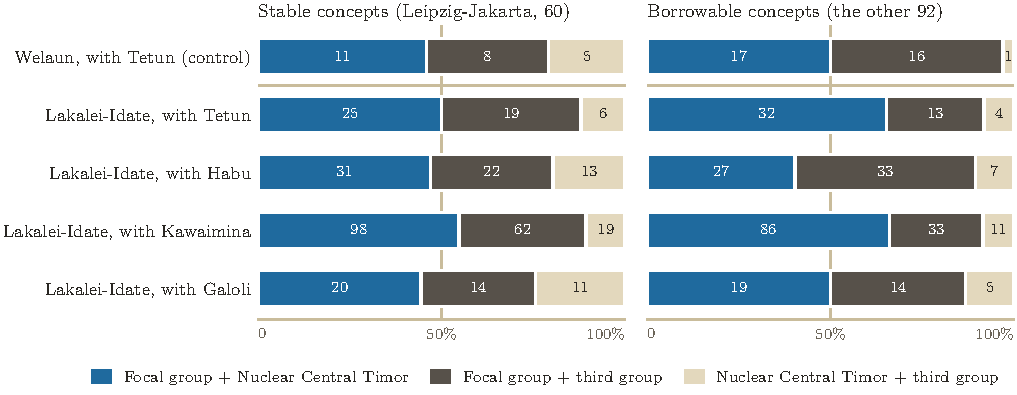
\includegraphics[width=\textwidth]{figures/triplets.pdf}
\caption{Triplet counts on stable (Leipzig-Jakarta) and borrowable concepts, with the original retention rule, representative lists. Each bar is one triplet of the focal group (Welaun or Lakalei-Idate), Nuclear Central Timor and a third group. Welaun, whose Tetun contact is documented, is the control: against a simulated null with unequal rates, only its jackknife Z in borrowable words stands out.}
\label{fig:S-triplets}
\end{figure}

\section{Sound changes}\label{sec:sound}

\begin{table}[tbp]
\caption{The eleven sound-change characters on the rival trees (E42),
with the root state free (Fitch) or fixed (Camin-Sokal,
Dollo).}
\label{tab:sound-steps}
\begin{tabularx}{\linewidth}{@{}L{1.72}L{0.68}L{0.8}L{0.8}@{}}
\toprule
\hd{Steps on each tree, rooted on Flores} & \hd{Lexical tree (H)} & \hd{Lakalei-Idate + Eastern Timor (G)} & \hd{Grimes and Edwards's split (GE)} \\
\midrule
*p lenition, Fitch & 2 & 2 & 2 \\
*p lenition, Camin-Sokal & 6 & 4 & 2 \\
*p lenition, Dollo & 2 & 2 & 2 \\
All eleven, Fitch & 33 & 34 & 32 \\
All eleven, Camin-Sokal & 49 & 47 & 51 \\
All eleven, Dollo & 54 & 49 & 43 \\
Lexical log-likelihood, relative to H & 0 & −10.5 & −12.0 \\
\bottomrule
\end{tabularx}
\end{table}

Several changes recur outside their defining groups: *ŋ \textgreater{} n throughout Timor-Babar and in Sika; *d \textgreater{} r, l in Sika and Dela; *p \textgreater{} h in Welaun; Hull's initial *b- \textgreater{} h in Galoli and Ili'uun. Lakalei-Idate also lacks Central Timor's *ŋ \textgreater{} g (*taliŋa `ear' \textgreater{} Idaté \emph{talina}, Mambae \emph{teliga}) and has *ma-p \textgreater{} b where Central Timor has *mp. Lacking Central Timor's change fits both trees if Lakalei-Idate branched off before Central Timor made it.

\textbf{A fuller phonology (E53).} Every non-retention reflex class in the expert atlas, kept if at least two of the 24 lects have it and two lack it, gives 36 characters. Under Camin-Sokal, G beats H on 6 characters to 0 (sign test p = 0.03), but all six are changes Tetun shares with Kawaimina and, where it is coded, Habu, and only two involve Lakalei-Idate; GE ties H. A Bayesian tree from these characters alone (binary Mk, coding=variable) recovers Lakalei-Idate (0.81) but neither of its placements, nor Timor-Babar (0.00 each). Combining sound-change characters with the lexical matrix at equal weight cannot show agreement, because the phonology is about 1\% of such a matrix \citep[on weighting character types, see][]{ringe2002}; a likelihood treatment of irreversible change, such as the stochastic Dollo model \citep{nicholls2008}, would need far more characters.

\section{Contact and linkage models}\label{sec:contact}

\textbf{Borrowing simulations (E21, E32).} Approximate Bayesian computation \citep{csillery2010} with borrowing from both sides into proto-Lakalei-Idate cannot separate the placements: the random forest \citep{pudlo2016} splits its votes 0.45 to 0.55 and misclassifies 36\% of its own simulations, and the four stable-vocabulary borrowing parameters end with posterior medians of 22 to 25\% and 90\% intervals of about 2 to 57\%, close to their U(0, 0.6) prior. The design's statistics are a handful of counts \citep{robert2011}, and its simulator moves both Lakalei-Idate lects together, so it cannot represent Idaté's and Lakalei's different neighbors.

\textbf{Glottometry (E22, E50).} Historical glottometry \citep{kalyan2018} finds cohesive groups only at low levels. With 95\% intervals from resampling concepts, Lakalei-Idate's subgroupiness is 1.42 (0 to 3.65), its ties to Central Timor 0.06 (0 to 0.31) and to Eastern Timor 0.08 (0 to 0.41), and Hull's Ramelaic 0 in every resample.

\textbf{A contact-aware tree (E19, E39).} contacTrees \citep{neureiter2022} did not settle when left free. Capped at five transfer edges, it used all five in every sample, some between unlikely partners (Dela and Habu in 99\% of samples). Its base tree puts Lakalei-Idate with Tetun and Habu (0.78), with a transfer edge between Lakalei and Tokodede in every sample. Because the model always uses the maximum number of edges it is misspecified, and its base tree should not be read as the history; it shows only that a few transfer events can carry the Central Timor signal as well as descent can. The run also mixed poorly (likelihood effective sample size 64), so its posterior shares are rough.

\textbf{A split network (E55).} NeighborNet \citep{bryant2004} on the primary distances, with 200 concept bootstraps, shows Lakalei-Idate as a split in 89\% of networks, Lakalei-Idate + Central Timor in 47\%, Idaté + Habu in 45\%, Lakalei + Nuclear Central Timor in 30\%, and Lakalei-Idate + Eastern Timor in 2\%. By the reading declared in advance this is ``unclear'': a linkage signature needed both sides in at least half of the networks.

\textbf{Correspondences (E33, E52).} Neither test can tell loans from inheritance in these lists. E33 finds the Lakalei items no closer to identity than inherited words. E52 found 0 to 2 regular non-identity correspondences per lect pair, from baselines of 24 to 30 shared retentions; of 18 decisive sets on each side, 5 were informative on the Central Timor side and 5 on the eastern side, splitting evenly between loan-like and inherited-like (Fisher p = 1.0 on both sides).

\section{Dating}\label{sec:dating}

Measured only in samples where both groups are clades (E49), the common ancestor of Lakalei-Idate and Central Timor is older than Central Timor's own by a median of 21\% of the latter's height under the relaxed clock (95\%: 4 to 71\%), where Central Timor with Welaun is a clade in 72\% of samples. Under the strict clock (E34), where both Nuclear Central Timor and Lakalei-Idate + Nuclear Central Timor are clades (49\% of samples), the second is older by a median of 21\% of the first's height (95\%: 7 to 39\%). Dropping Tela-Masbuar moves the relaxed clock's root mass from Kisar-Luang toward the western branches (E41).

\section{Welaun (C2)}\label{sec:welaun}

On the 60 stable concepts Welaun + Tetun gets 2\% (UPGMA) and 4\% (NJ), on the other 92 concepts 74\% and 81\% (E1), and the triplet test locates the excess there (Z = 6.9 against 0.6). Under the consensus coding the Welaun control's tree pair becomes Welaun + Tetun even on stable concepts (10 to 8). Under the strict clock (E34) Central Timor with Welaun has posterior 0.29. \citet{hull2003} called Bekais a distinct language ``structurally intermediate between Belunese Tetum and Dawan'' (in the article's English abstract).

\section{Other disputed branches}\label{sec:branches}

\begin{table}[H]
\caption{Triplet tests on other disputed placements (E24), with the
original retention rule; rule R2 gives the same largest pair in every
triplet. The imbalances between the other two pairs are uncalibrated for
these triplets and none survives multiple-testing correction, so they
are not read as contact.}
\label{tab:branches}
\begin{tabularx}{\linewidth}{@{}L{0.6}L{1.543}L{0.857}@{}}
\toprule
\hd{Triplet} & \hd{Counts, all concepts (stable)} & \hd{Reading} \\
\midrule
Habu, Tetun, Kawaimina & Habu+Tetun 15 (5); Habu+Kawaimina 11 (5); Tetun+Kawaimina 4 (2) & Unresolved \\
Waima'a, Naueti, Midiki & Waima'a+Naueti 10 (7); Waima'a+Midiki 7 (4); Naueti+Midiki 2 (1) & Waima'a+Naueti largest, as in Grimes and Edwards \\
Galoli, Wetar, Dadu'a & Galoli+Dadu'a 20 (13); Galoli+Wetar 6 (2); Wetar+Dadu'a 6 (4) & Galoli+Dadu'a largest \\
Galoli, Wetar, Tetun & Galoli+Wetar 12 (8); Galoli+Tetun 6 (4); Wetar+Tetun 0 (0) & Galoli+Wetar largest \\
Helong, Meto, Rote & Meto+Rote 17 (12); Helong+Meto 10 (8); Helong+Rote 3 (2) & Meto+Rote largest \\
\bottomrule
\end{tabularx}
\end{table}

\end{document}
